% vim: spell spelllang=en_gb
\chapter{Results}

This section presents the results of the methods used by evaluating each step of the pipeline: (1)
classifying flood-relevant tweets, (2) extracting geographical locations from tweets, (3) finding
useful insights using textual analysis techniques, and (4) visualizing the results in a searchable
matter.

\section{Text Classification}
Table~\ref{tab:metrics} shows the evaluation metrics mention in
Section~\ref{sec:text_classification_section} for the trained DistilBERT model on the dataset and a
balanced version by doing undersampling using imblanaced-learn's RandomUnderSampler
method\footnote{https://imbalanced-learn.org/stable/references/generated/imblearn.under\_sampling.RandomUnderSampler.html}.
Table~\ref{tab:tweets_missclassified} shows falsely classified tweets from the Swedish dataset
translated to English.

\begin{table}
  \center
  \bgroup
  \def\arraystretch{1.5}
  \begin{tabular}{|c|c|c|c|c|c|}
    \hline
            & Accuracy & Precision & Recall & F$_1$ Score & Confusion Matrix\\
            \hline
    Original & 0.9231 & 0.8944 & 0.9181 & 0.9061 &
    $
    \begin{bmatrix}
      381 & 34 \\ 
      568 & 45
    \end{bmatrix}
    $\\
    \hline
    Undersampled & 0.9137 & 0.9091 & 0.9138 & 0.9115 &
    $
    \begin{bmatrix}
      350 & 33\\ 
      370 & 35
    \end{bmatrix}
    $\\
    \hline
  \end{tabular}
  \egroup
  \caption{Evaluation metrics}
  \label{tab:metrics}
\end{table}

\begin{table}
  \center
  \begin{tabular}{|p{5cm}|p{5cm}|l|l|}
    \hline
    Translated tweet & Processed tweet & Predicted label & Actual label\\
    \hline
    The road has rained away outside our driveway!! Damn storm https://t.co/wU6uuZo7El &
    road rained away outside driveway damn storm & 0 & 1 \\
    \hline
    Right now! Stormy weather in southern Norway. Functionality affected - all resources prioritized to save lives, correct in Vestfold. &
    right stormy weather southern norway functionality affected resources prioritized save lives correct vestfold & 0 & 1\\
    \hline
    AFTER LIGHT! Basement full of water? Do you live in \#Stockholm and are affected by this weekend's
    \#flooding? Call reporter Nadya bums &
    light basement water live affected weekends reporter nadya bums & 0 & 1\\
    \hline
    Impressed by efforts and people's patience. Here is the latest municipal information. \#Hallsberg
    \#Flooding \#orepol \#svpol http://t.co/C0sCxEDtLT &
    impressed efforts peoples patience latest municipal information & 0 & 1 \\
    \hline
    world Floods, war, famine, terror. Goodnight world. & 
    floods war famine terror goodnight & 1 & 0 \\
    \hline
    Flooding in the bathtub? & 
    flooding bathtub & 1 & 0 \\
    \hline
    A basement was flooded when a water main leaked in \#Vårberga in \#Borgå \#borgåvatten https://t.co/zX08QDqJv9 & 
    basement flooded water main leaked & 1 & 0 \\
    \hline
    storm flood assumption years Storm flood assumption off by about 2,500 years https://t.co/v14XtEcbTC & 
    storm flood assumption years & 1 & 0 \\
    \hline
  \end{tabular}
  \caption{Miss-classified tweets}
  \label{tab:tweets_missclassified}
\end{table}


\section{Experiments}%
\label{sec:Experiments}

This section presents the results by applying the pipeline to three unlabelled collections and
showing the most noteworthy results from the visualizations. One week's worth of tweets are
extracted from Twitter's API starting from the date of the beginning of the events using a query
created by experts at a workshop in \ac{SMHI} containing flood-relevant terms in Swedish:

\begin{verbatim}
 "atmosfärisk flod" OR "hög vatten" OR åskskur
 OR regnskur OR dagvattensystem OR dränering OR "höga vågor"
 OR "höga flöden" OR dämmor
 OR snösmältning OR blött OR oväder OR stormflod OR vattenstånd
 OR vattennivå OR åskväder OR regnstorm"
 OR "mycket regn" OR "kraftig regn" OR översvämningsskador
 OR översvämningar OR översvämning
\end{verbatim}

Gävleborg and Dalarna counties had a flood event on the 18th of
August\footnote{https://floodlist.com/europe/central-sweden-floods-august-2021} damaging their
infrastructure, such as houses and roads. After extracting and processing the tweets, 910 are left,
of which 700 are classified as flood-relevant. The classifier seems to have high precision, yet it
has some low recall. Table~\ref{tab:tweets_missclassified_gavle} shows some of the false negatives.

\begin{table}
  \center
  \begin{tabular}{|p{7.5cm}|p{7.5cm}|}
    \hline
    Translated tweet & Processed tweet\\
    \hline
    Ovädret och det kraftiga regnandet i Gävle har tvingat Brynäs att stänga sin hemmaarena på grund av
    översvämning. \#twittpuck \#Brynäs https://t.co/hrZA9icAy7 &
    Ovädret and the heavy rains in Gävle have forced Brynäs to close its home on the ground of
    overturning. \#twittpuck \#Brynäs https://t.co/hrZA9icAy7 \\
    \hline
    Blött i Gävle sa Bull.. https://t.co/fV1ChW7ZTR &
    Wet in Gävle said Bull.. https://t.co/fV1ChW7ZTR \\
    \hline
    Att tänka på mycket regn bakåt i tiden o tänka på bl.a. ån i Halland som steg o ställde till det !&
    Thinking about a lot of rain back in time and thinking about e.g. the river in Halland that rose and
    made it happen! \\
    \hline
    Nån som vet om det är lite blött i Gävle?&
    Anyone know if it's a bit wet in Gävle? \\
    \hline
  \end{tabular}
  \caption{Miss-classified tweets for floods in Gävleborg and Dalarna}
  \label{tab:tweets_missclassified_gavle}
\end{table}

Figure~\ref{fig:gavle_map} shows 114 identified locations in Gävleborg county tweets, such as Gävle (96), and
according to the histogram in Figure~\ref{fig:gavle_histogram}, 81 out of the 114 tweets were created on the 18th of August,
22 on the 19th, and 6 on the 20th. Some locations are identified incorrectly, such as:
\begin{itemize}
  \item \textbf{Original tweet}: Dödssiffran stiger i turkiska översvämningar \#Turkiet \#svpol
    https://t.co/K6kLRmxQdw \\
  \textbf{Translated tweet}: Death toll rises in Turkish floods \#Turkey \#svpol \\
    https://t.co/K6kLRmxQdw \\
    \textbf{Identified location}: Turkiet, a hamlet\footnote{isolated settlement} in Uppsala county. \\
    \textbf{Actual location}: Turkey, the country.

  \item \textbf{Original tweet}: Information. Det kraftiga regnovädret över Gävle har orsakat
    översvämningar i arenan. Detta innebär att all verksamhet i Monitor ERP Arena, vilket inkluderar
    bland annat aktivitet på isen samt restaurangverksamheten, tills vidare är pausad. Vi återkommer
    med mer information. https://t.co/gHDfirq9VS \\
    \textbf{Translated tweet}: Information. The heavy rain over Gävle has caused flooding in the arena.
    This means that all activities in the Monitor ERP Arena, which includes activities on the ice as
    well as restaurant operations, are paused until further notice. We will return with more
    information. https://t.co/gHDfirq9VS \\
    \textbf{Identified location}: Årena, an isolated dwelling\footnote{consist of not more than 2 households}
    in Kalmar county. \\
    \textbf{Actual location}: Gävle.


\end{itemize}

\begin{figure}[H]
  \begin{center}
    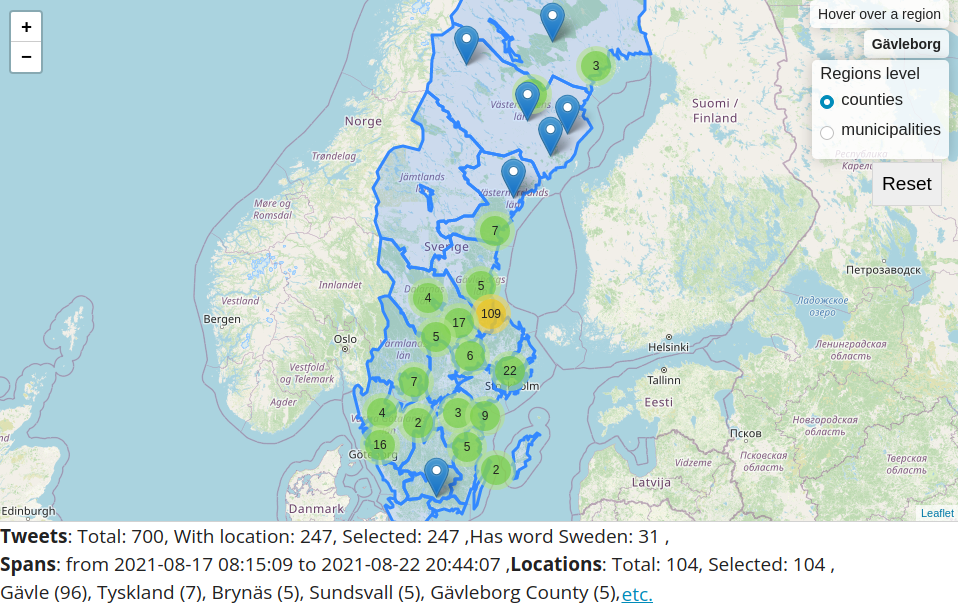
\includegraphics[width=\columnwidth]{./images/gavle_map.png}
  \end{center}
  \caption{Map showing tweets about flood event in Gävleborg}
  \label{fig:gavle_map}
\end{figure}

\begin{figure}[H]
  \begin{center}
    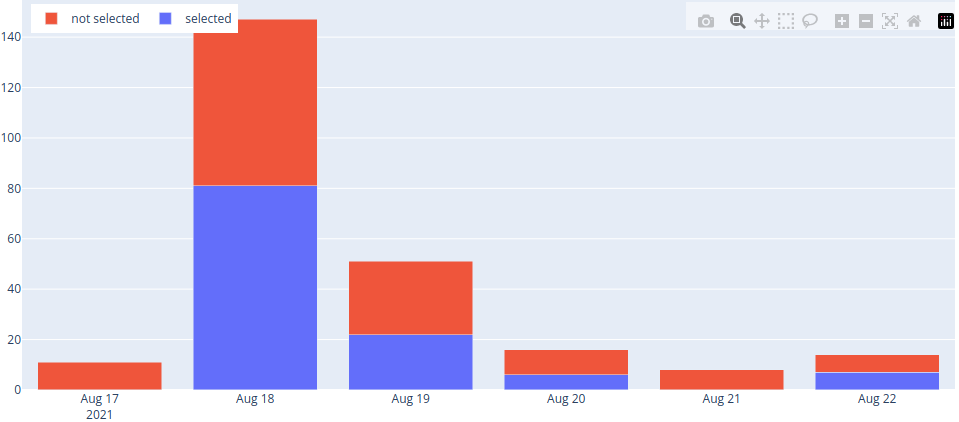
\includegraphics[width=\columnwidth]{./images/gavle_histogram.png}
  \end{center}
  \caption{Histogram showing tweets about flood event in Gävleborg}
  \label{fig:gavle_histogram}
\end{figure}


Figure~\ref{fig:gavle_text_analysis} shows the scatter plot, the tweet table and the \ac{LDA} table after only considering a
cluster of tweets in the bottom left of the scatter plot, and they are discussing traffic
disruption.

\begin{figure}[H]
  \begin{center}
    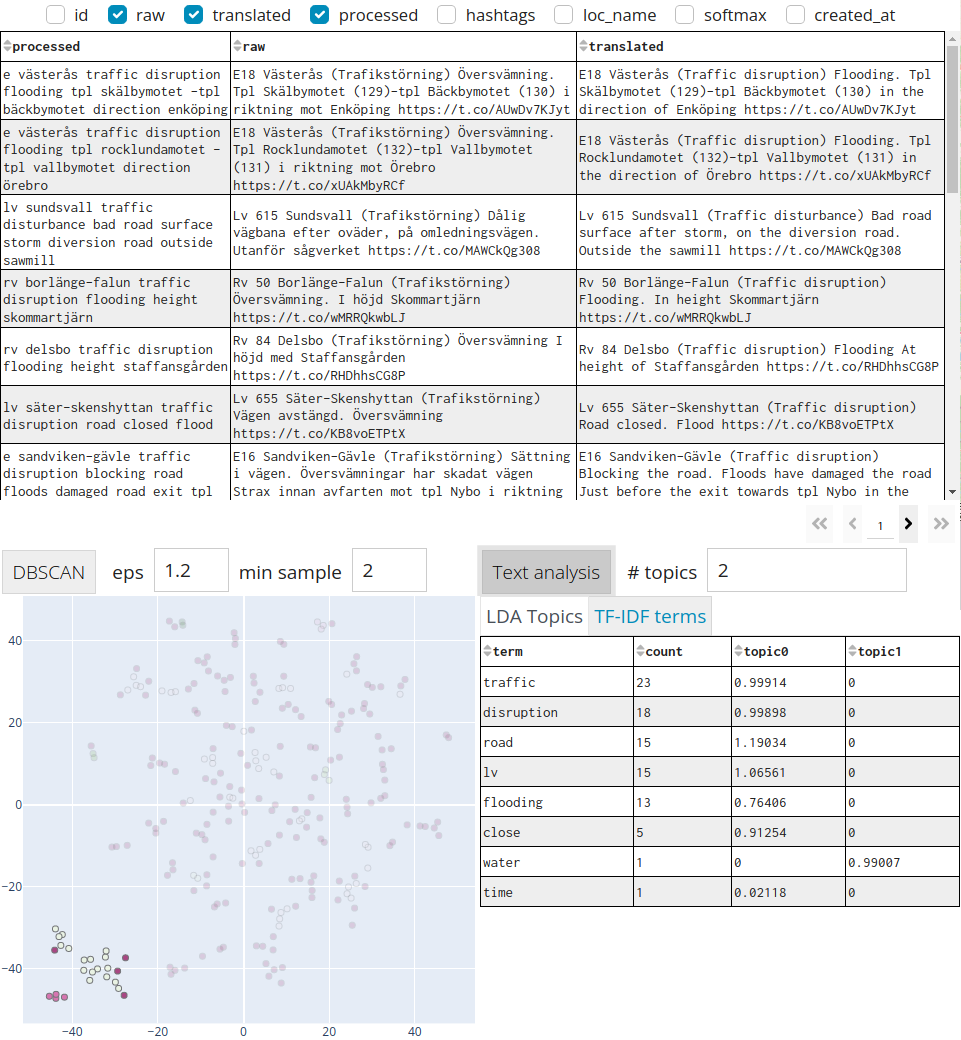
\includegraphics[width=\columnwidth]{./images/gavle_text_analysis.png}
  \end{center}
  \caption{Tweet table, scatter plot, and \ac{LDA} table showing a cluster of tweets about flood event in Gävleborg}
  \label{fig:gavle_text_analysis}
\end{figure}


Heavy rain caused flooding in Gothenburg on 11 September
2019\footnote{https://floodlist.com/europe/sweden-flash-floods-gothenburg-september-2019}.
Figure~\ref{fig:gothenburg_map}
shows that there are 18 flood-relevant tweets in Gothenburg county, of which 12 were created on the
11th and three on the 12th.  There are 16 tweets containing Spanien and identifying it as an
isolated dwelling in Stockholm which is incorrect; the tweets are discussing floods in the country
Spain\footnote{https://www.svt.se/nyheter/utrikes/stora-oversvamningar-har-drabbat-sodra-spanien}. There
are false negatives for classifying flood-relevant tweets, such as ``It was a little
wet. https://t.co/PcroA3s1A2'', where the tweet contains a \ac{URL} for an article mentioning the
flood event.

\begin{figure}[H]
  \begin{center}
    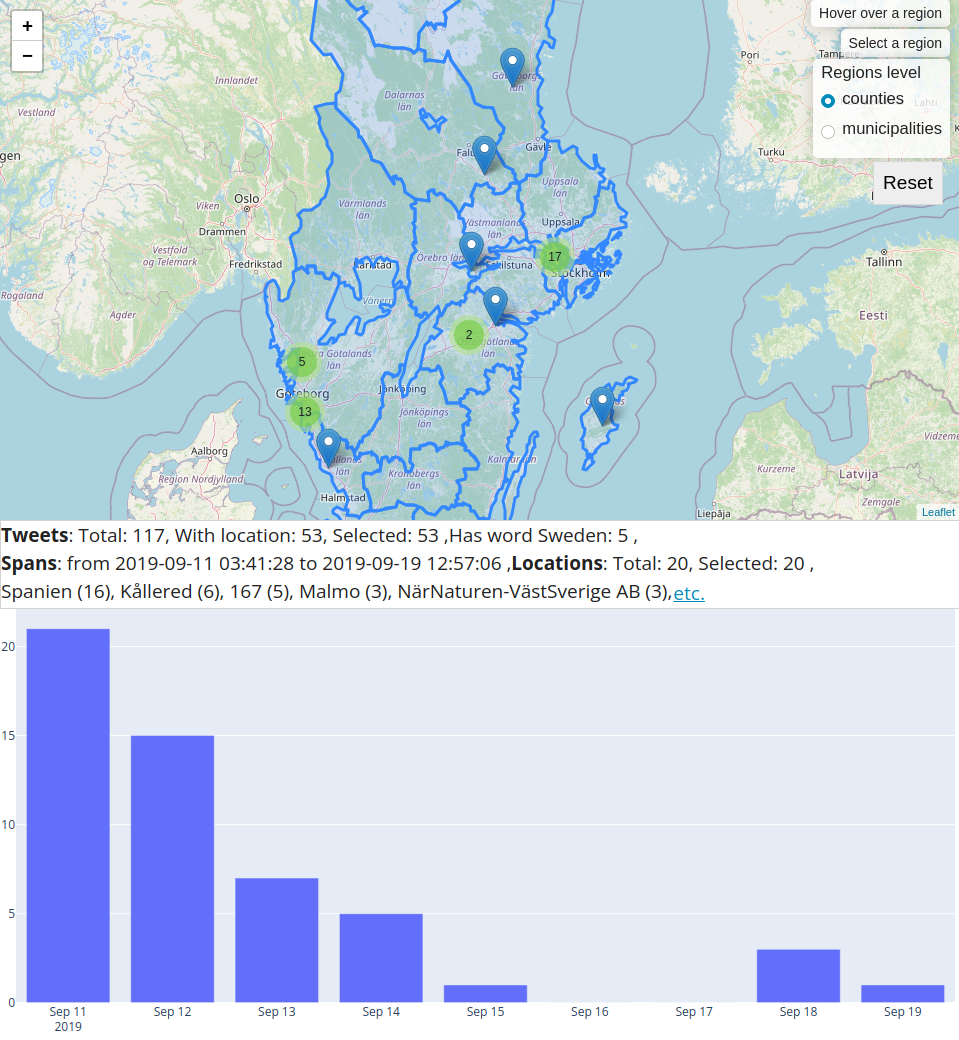
\includegraphics[width=\columnwidth]{./images/gothenburg_floods.png}
  \end{center}
  \caption{Tweet table  showing tweets about flood event in Gothenburg}
  \label{fig:gothenburg_map}
\end{figure}

On 22 August 2014, Halland, Värmland and Västra Götaland counties had floods lasting four days
caused by heavy rain. The map in Figure~\ref{fig:4days_floods} shows that Halland, Värmland, and Västra Götaland counties
have 11, 24, and 8 tweets, respectively. The histogram shows eight tweets created on the 22nd of the
month and 12 on the 23rd.

\begin{figure}[H]
  \begin{center}
    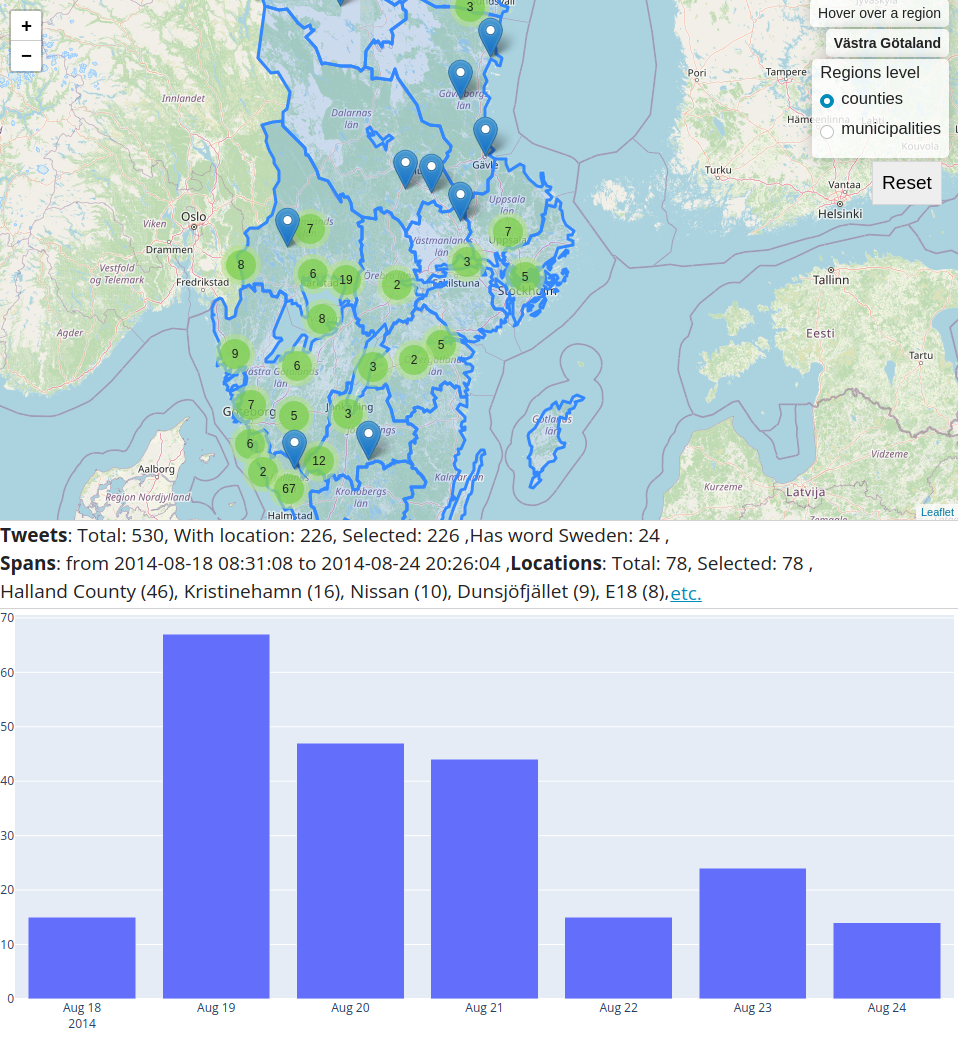
\includegraphics[width=\columnwidth]{./images/4days_floods.png}
  \end{center}
  \caption{Map and histogram showing tweets about flood event in Swedish counties}
  \label{fig:4days_floods}
\end{figure}

The bottom left cluster in the scatter plot shown in Figure~\ref{fig:4days_text_analysis} contains tweets discussing \ac{SMHI}
warnings.

\begin{figure}[H]
  \begin{center}
    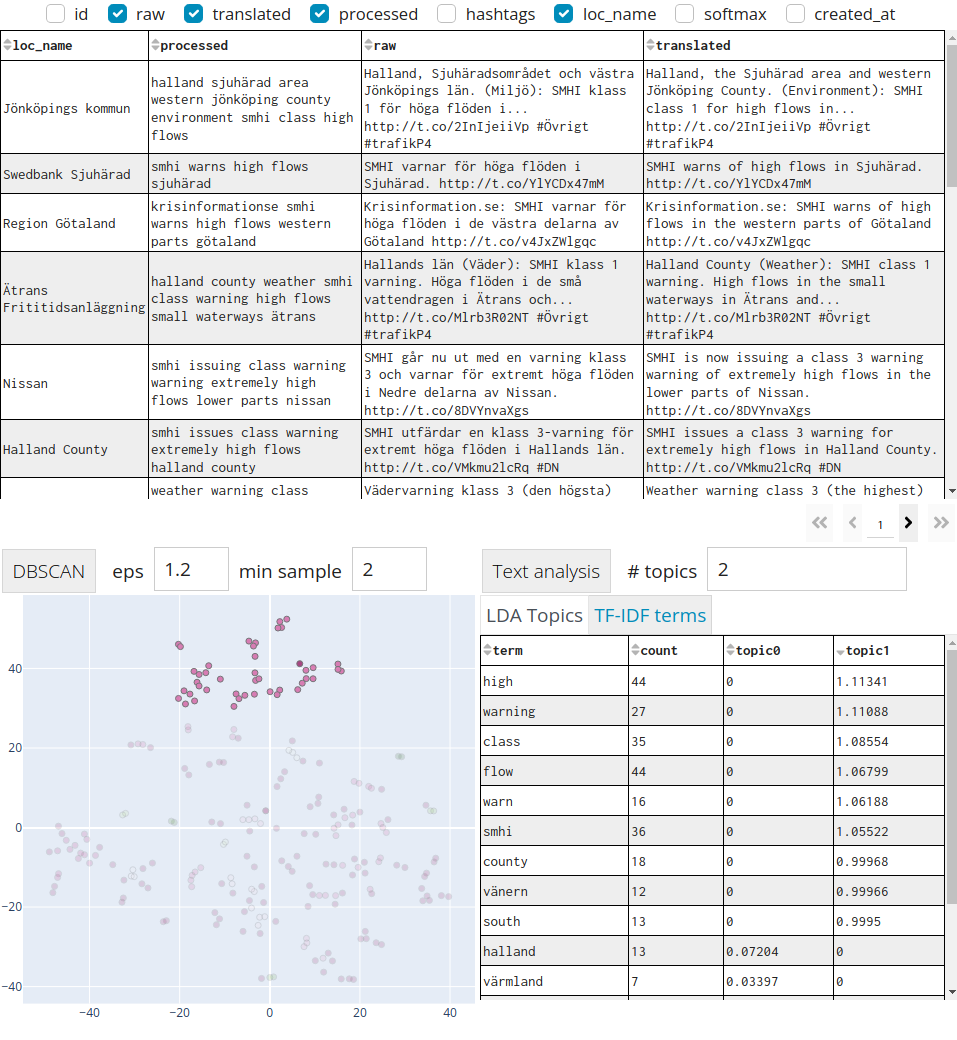
\includegraphics[width=\columnwidth]{./images/4days_text_analysis.png}
  \end{center}
  \caption{Tweet table, scatter plot, and \ac{LDA} table showing a cluster of tweets about flood
  event in Swedish counties}
  \label{fig:4days_text_analysis}
\end{figure}
